% FIG:q03-emissions
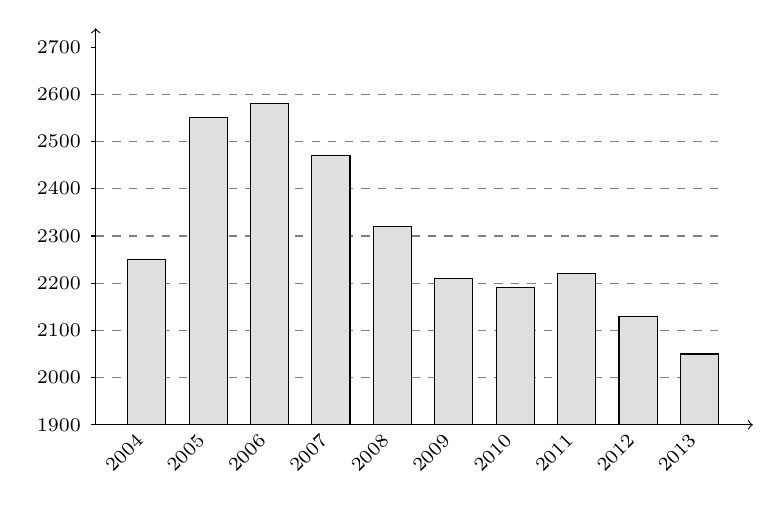
\begin{tikzpicture}[x=0.78cm,y=0.006cm,line width=0.4pt]
  % Approximate bar heights transcribed from the source image, not exact data.
  \draw[->] (0,1900) -- (10.7,1900);
  \draw[->] (0,1900) -- (0,2740);
  \foreach \y in {1900,2000,...,2700} {
    \draw (0,\y) -- (-0.08,\y) node[left] {\scriptsize \y};
  }
  \foreach \y in {2000,2100,...,2600} {
    \draw[dashed,gray] (0,\y) -- (10.2,\y);
  }
  \draw (0,1900) -- (10.2,1900);
  \foreach \i/\year/\v in {
    0/2004/2250,1/2005/2550,2/2006/2580,3/2007/2470,4/2008/2320,
    5/2009/2210,6/2010/2190,7/2011/2220,8/2012/2130,9/2013/2050} {
    \pgfmathsetmacro{\x}{0.52+\i}
    \draw[fill=gray!25] (\x,1900) rectangle ++(0.62,\v-1900);
    \node[below=2pt,rotate=45,anchor=east] at (\x+0.31,1900) {\scriptsize \year};
  }
\end{tikzpicture}
